\subsection{A trained shared generator and simultaneous validation}\label{sec:learned-experiment}
We now learn the conditional generator for \eqref{eq:synthetic-field}. The model is \eqref{eq:neural-detail} with twelve hidden units, a softmax vector of positive output weights, and a learned positive innovation scale. It has 37 trainable parameters shared across every mode. The first mode is sampled exactly. Each hidden row is projected onto the Euclidean ball of radius $1.3$ after every update; the innovation scale is constrained to $[0.7,1.3]$.

For each of three preselected seeds, training uses 8,192 independent noisy target fields observed through mode 32. There are 1,800 Adam steps of 2,048 context/detail pairs, with learning rate $0.012$. Half the sampled pairs use mode 2 and the rest sample modes 3--32 uniformly. The objective is Gaussian conditional negative log-likelihood for the normalized coefficient $jU_j$. Conditional means are not supplied as training labels. There is no validation-based hyperparameter or seed selection.

An independent audit contains 65,536 fields through mode 256. Because the synthetic conditional mean is known, it evaluates the bounded loss in \Cref{sec:validation} with $B_j=4$. The $K=3$ candidate networks and all 255 detail modes share an overall failure probability $\delta=0.01$. The global sensitivity uses the actual learned value $K_\theta=\sum_kp_k\|a_k\|$, not a Jacobian measured at a few validation points. The values for the three runs are $0.966423$, $0.965939$, and $1.024007$; their innovation scales are $0.994923$, $1.005759$, and $0.985614$.

\begin{table}[htbp]
\centering\small
\begin{tabular}{rrrrr}
\toprule
Modes & Coupling RMS & Estimated $d_m$ & 99\% $d_m$ & 99\% full-law bound \\
\midrule
8 & 0.36176 & 0.01201 & 0.04367 & 0.48676 \\
16 & 0.25508 & 0.01283 & 0.04824 & 0.35143 \\
32 & 0.17553 & 0.01323 & 0.05065 & 0.25318 \\
64 & 0.11550 & 0.01343 & 0.05189 & 0.18357 \\
128 & 0.06724 & 0.01352 & 0.05251 & 0.13536 \\
256 & 0.00908 & 0.01357 & 0.05283 & 0.10290 \\
\bottomrule
\end{tabular}

\caption{The first preselected training seed. Coupling RMS is an empirical cost to the 256-mode target reference, and estimated $d_m$ plugs empirical conditional errors into the recurrence. The last two columns use simultaneous 99-percent conditional-error bounds; only the final column also includes the infinite target tail.}\label{tab:learned}
\end{table}

At mode 256, the empirical projected coupling RMS is respectively $0.009081$, $0.006697$, and $0.025350$. The full-law confidence bounds are $0.102899$, $0.102447$, and $0.109925$. The distinction is material: the conservative unresolved target-tail bound alone is $0.088302$, and statistical confidence also enlarges the conditional-error inputs. The standard errors of the squared coupling costs are recorded in the numerical file; they do not replace the population confidence calculation.

A separately retrained ablation removes the previous-band input while retaining the first coordinate. Its 256-mode coupling RMS is $0.105823$. Removing all mean context, while preserving the target innovation scale, gives $0.417298$. These controlled ablations isolate the value of conditional information within the stated field model. They do not rank this architecture against diffusion models or neural operators trained on other datasets.

\begin{figure}[tb]
\centering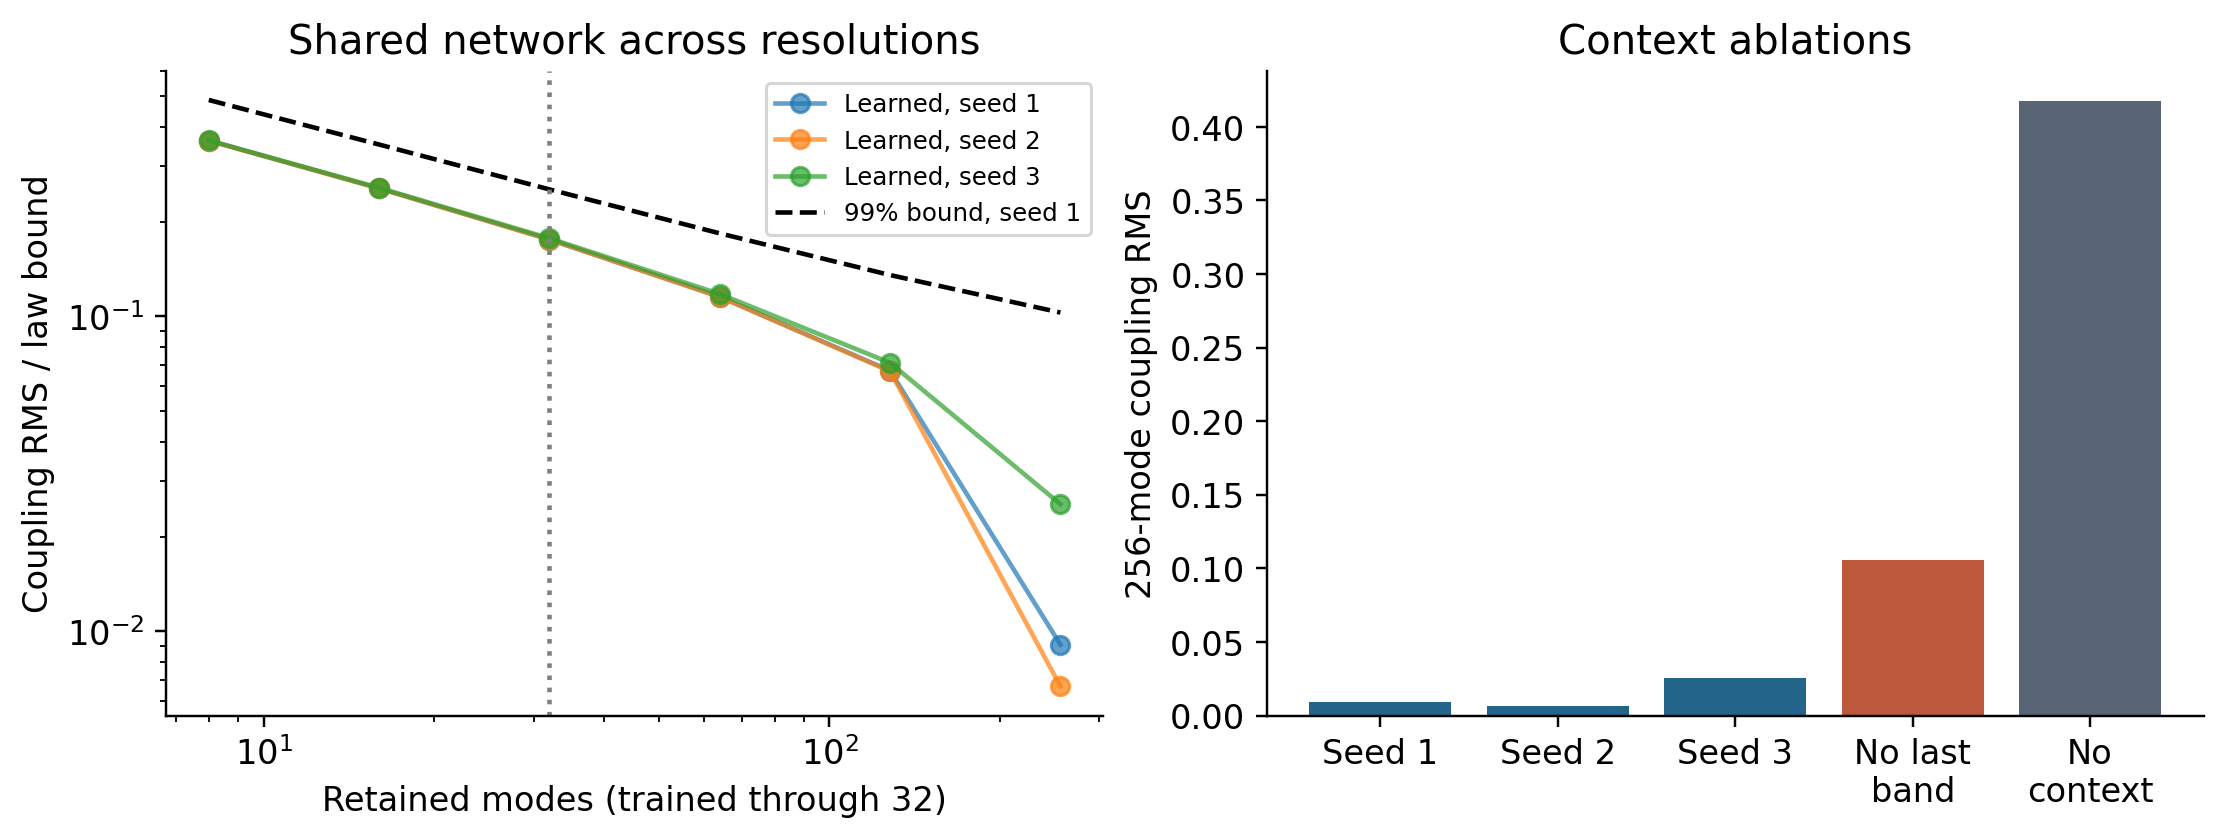
\includegraphics[width=\textwidth]{figures/learned_operator.png}
\caption{A neural model trained through 32 modes and audited through 256. The left panel distinguishes empirical finite-reference coupling costs from the first seed's full-law confidence bound. The right panel compares all three seeds with context ablations. Shared innovations reproduce every retained coefficient exactly when additional modes are requested.}\label{fig:learned}
\end{figure}

The supplied CPU float64 program records every training seed, objective, constraint, fitted parameter, bandwise fitting estimate, confidence input, and context bound. The audit uses new target fields beyond the training cutoff, so this experiment tests resolution extrapolation with known conditional laws. It does not claim that unobserved fine-scale laws can be inferred from coarse data without the structural assumptions stated in the model.
